\documentclass[journal, a4paper]{IEEEtran}

\usepackage[utf8x]{inputenc}
\usepackage[francais]{babel}

\usepackage{listings}

% some very useful LaTeX packages include:

%\usepackage{cite}      % Written by Donald Arseneau
                        % V1.6 and later of IEEEtran pre-defines the format
                        % of the cite.sty package \cite{} output to follow
                        % that of IEEE. Loading the cite package will
                        % result in citation numbers being automatically
                        % sorted and properly "ranged". i.e.,
                        % [1], [9], [2], [7], [5], [6]
                        % (without using cite.sty)
                        % will become:
                        % [1], [2], [5]--[7], [9] (using cite.sty)
                        % cite.sty's \cite will automatically add leading
                        % space, if needed. Use cite.sty's noadjust option
                        % (cite.sty V3.8 and later) if you want to turn this
                        % off. cite.sty is already installed on most LaTeX
                        % systems. The latest version can be obtained at:
                        % http://www.ctan.org/tex-archive/macros/latex/contrib/supported/cite/

\usepackage{graphicx}   % Written by David Carlisle and Sebastian Rahtz
                        % Required if you want graphics, photos, etc.
                        % graphicx.sty is already installed on most LaTeX
                        % systems. The latest version and documentation can
                        % be obtained at:
                        % http://www.ctan.org/tex-archive/macros/latex/required/graphics/
                        % Another good source of documentation is "Using
                        % Imported Graphics in LaTeX2e" by Keith Reckdahl
                        % which can be found as esplatex.ps and epslatex.pdf
                        % at: http://www.ctan.org/tex-archive/info/

%\usepackage{psfrag}    % Written by Craig Barratt, Michael C. Grant,
                        % and David Carlisle
                        % This package allows you to substitute LaTeX
                        % commands for text in imported EPS graphic files.
                        % In this way, LaTeX symbols can be placed into
                        % graphics that have been generated by other
                        % applications. You must use latex->dvips->ps2pdf
                        % workflow (not direct pdf output from pdflatex) if
                        % you wish to use this capability because it works
                        % via some PostScript tricks. Alternatively, the
                        % graphics could be processed as separate files via
                        % psfrag and dvips, then converted to PDF for
                        % inclusion in the main file which uses pdflatex.
                        % Docs are in "The PSfrag System" by Michael C. Grant
                        % and David Carlisle. There is also some information
                        % about using psfrag in "Using Imported Graphics in
                        % LaTeX2e" by Keith Reckdahl which documents the
                        % graphicx package (see above). The psfrag package
                        % and documentation can be obtained at:
                        % http://www.ctan.org/tex-archive/macros/latex/contrib/supported/psfrag/

%\usepackage{subfigure} % Written by Steven Douglas Cochran
                        % This package makes it easy to put subfigures
                        % in your figures. i.e., "figure 1a and 1b"
                        % Docs are in "Using Imported Graphics in LaTeX2e"
                        % by Keith Reckdahl which also documents the graphicx
                        % package (see above). subfigure.sty is already
                        % installed on most LaTeX systems. The latest version
                        % and documentation can be obtained at:
                        % http://www.ctan.org/tex-archive/macros/latex/contrib/supported/subfigure/

\usepackage{url}        % Written by Donald Arseneau
                        % Provides better support for handling and breaking
                        % URLs. url.sty is already installed on most LaTeX
                        % systems. The latest version can be obtained at:
                        % http://www.ctan.org/tex-archive/macros/latex/contrib/other/misc/
                        % Read the url.sty source comments for usage information.

%\usepackage{stfloats}  % Written by Sigitas Tolusis
                        % Gives LaTeX2e the ability to do double column
                        % floats at the bottom of the page as well as the top.
                        % (e.g., "\begin{figure*}[!b]" is not normally
                        % possible in LaTeX2e). This is an invasive package
                        % which rewrites many portions of the LaTeX2e output
                        % routines. It may not work with other packages that
                        % modify the LaTeX2e output routine and/or with other
                        % versions of LaTeX. The latest version and
                        % documentation can be obtained at:
                        % http://www.ctan.org/tex-archive/macros/latex/contrib/supported/sttools/
                        % Documentation is contained in the stfloats.sty
                        % comments as well as in the presfull.pdf file.
                        % Do not use the stfloats baselinefloat ability as
                        % IEEE does not allow \baselineskip to stretch.
                        % Authors submitting work to the IEEE should note
                        % that IEEE rarely uses double column equations and
                        % that authors should try to avoid such use.
                        % Do not be tempted to use the cuted.sty or
                        % midfloat.sty package (by the same author) as IEEE
                        % does not format its papers in such ways.

\usepackage{amsmath}    % From the American Mathematical Society
                        % A popular package that provides many helpful commands
                        % for dealing with mathematics. Note that the AMSmath
                        % package sets \interdisplaylinepenalty to 10000 thus
                        % preventing page breaks from occurring within multiline
                        % equations. Use:
%\interdisplaylinepenalty=2500
                        % after loading amsmath to restore such page breaks
                        % as IEEEtran.cls normally does. amsmath.sty is already
                        % installed on most LaTeX systems. The latest version
                        % and documentation can be obtained at:
                        % http://www.ctan.org/tex-archive/macros/latex/required/amslatex/math/



% Other popular packages for formatting tables and equations include:

%\usepackage{array}
% Frank Mittelbach's and David Carlisle's array.sty which improves the
% LaTeX2e array and tabular environments to provide better appearances and
% additional user controls. array.sty is already installed on most systems.
% The latest version and documentation can be obtained at:
% http://www.ctan.org/tex-archive/macros/latex/required/tools/

% V1.6 of IEEEtran contains the IEEEeqnarray family of commands that can
% be used to generate multiline equations as well as matrices, tables, etc.

% Also of notable interest:
% Scott Pakin's eqparbox package for creating (automatically sized) equal
% width boxes. Available:
% http://www.ctan.org/tex-archive/macros/latex/contrib/supported/eqparbox/

% *** Do not adjust lengths that control margins, column widths, etc. ***
% *** Do not use packages that alter fonts (such as pslatex).         ***
% There should be no need to do such things with IEEEtran.cls V1.6 and later.


% Your document starts here!
\begin{document}

% Define document title and author
	\title{Administration des réseaux}
	\author{Alexandre Kervadec
	\thanks{Professeur : A.Guermouche}}
	\markboth{Université de Bordeaux - Master 1 Informatique}{}
	\maketitle

% Write abstract here
\begin{abstract}
	Notes du cours d'administration des réseaux de A.Guermouche
\end{abstract}

% Each section begins with a \section{title} command
\section{Modèle TCP/IP}
	% \PARstart{}{} creates a tall first letter for this first paragraph
	\subsection{Le visage d'internet}
	\begin{itemize}
		\item Une construction à partir du "bas"
		\begin{itemize}
			\item réseau local (laboratoire, département)
			\item réseau local (campus, entreprise)
			\item réseau régional
			\item réseau national
			\item réseau mondial
		\end{itemize}
		\item 3 niveaux d'interconnexion
		\begin{itemize}
			\item postes de travail (ordinateur, terminal, ...)
			\item liaisons physiques (câble, fibre, RTC, ...)
			\item routeurs (équipement spécialisé, ordinateur, ...)
		\end{itemize}
	\end{itemize}
	C'est un ensemble de sous-réseaux indépendants (Autonomous System) et hétérogènes qui sont inter-connectés (organisation hiérarchique)
	
	\begin{figure}[!hbt]
		\begin{center}
		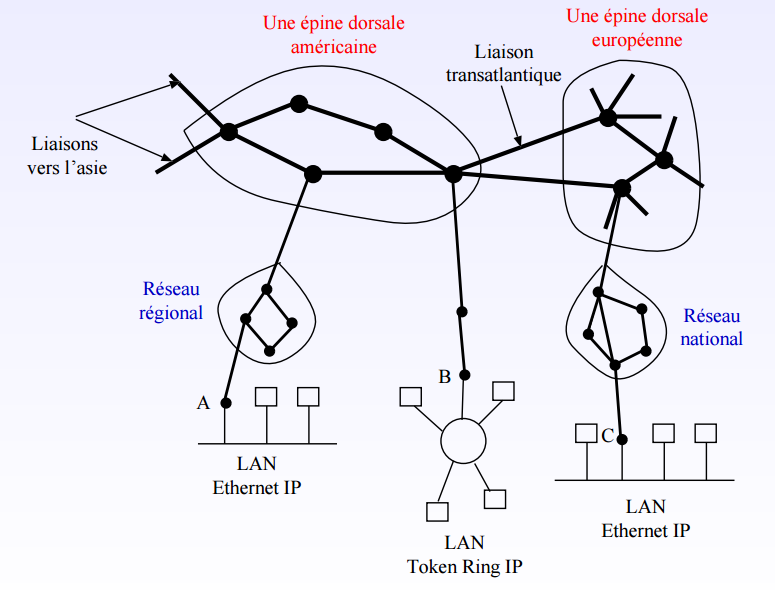
\includegraphics[width=\columnwidth]{orga_hier.png}
		\label{fig:orga_hier}
		\end{center}
	\end{figure}
	
	\subsection{Architecture TCP/IP}
	L'architecture TCP/IP est une version simplifiée du modèle OSI.
	\begin{itemize}
		\item \textbf{Application} : FTP, WWW, Telnet, SMTP, ...
		\item \textbf{Transport} : TCP, UDP (entre 2 processus aux extrémités)
		\begin{itemize}
			\item TCP : transfert fiable de données en mode connecté
			\item UDP : transfert non garanti de données en mode non-connecté
		\end{itemize}
		\item \textbf{Réseau} : IP (routage)
		\item \textbf{Physique} : transmission entre 2 sites
		\begin{itemize}
			\item TCP : Transport Control Protocol
			\item UDP : User Datagram Protocol
			\item IP : Internet Protocol
		\end{itemize}
 	\end{itemize}
	
	\begin{figure}[!hbt]
		\begin{center}
		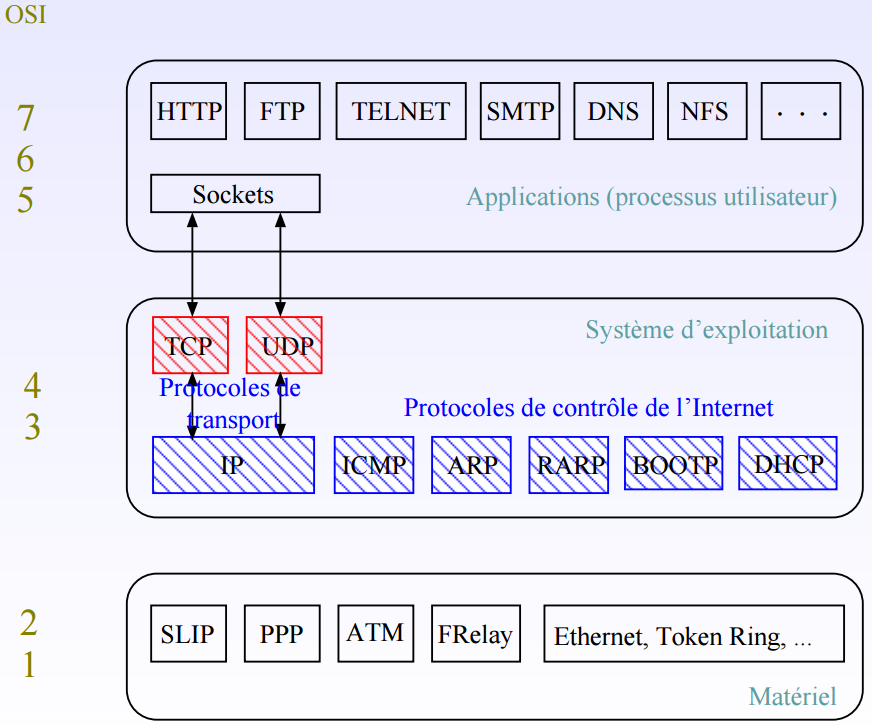
\includegraphics[width=\columnwidth]{archi_tcp_ip.png}
		\caption{Architecture TCP/IP}
		\label{fig:archi_tcp_ip}
		\end{center}
	\end{figure}
	
	\begin{figure}[!hbt]
		\begin{center}
		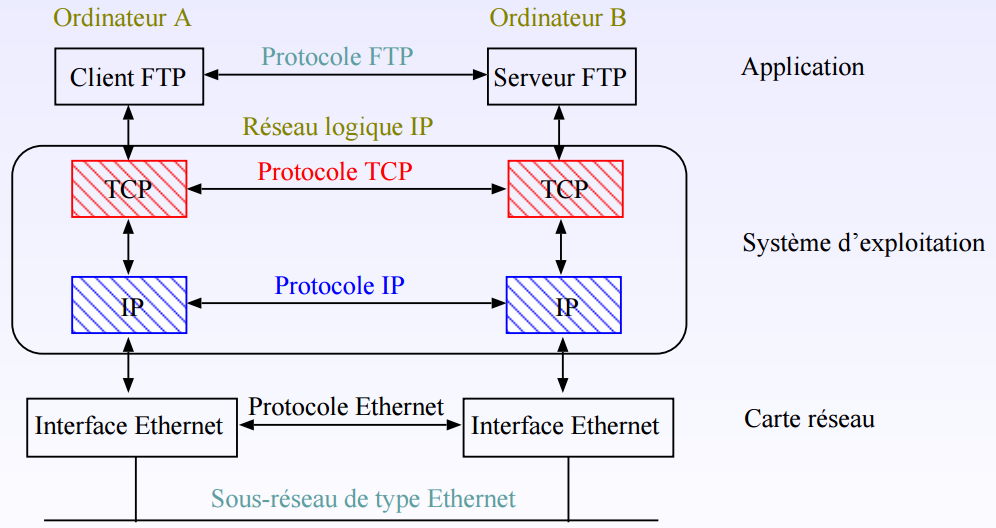
\includegraphics[width=\columnwidth]{sous_res_ip.png}
		\caption{Sous-réseau IP}
		\label{fig:sous_res_ip}
		\end{center}
	\end{figure}
	
	\newpage
	
	\begin{figure}[!hbt]
		\begin{center}
		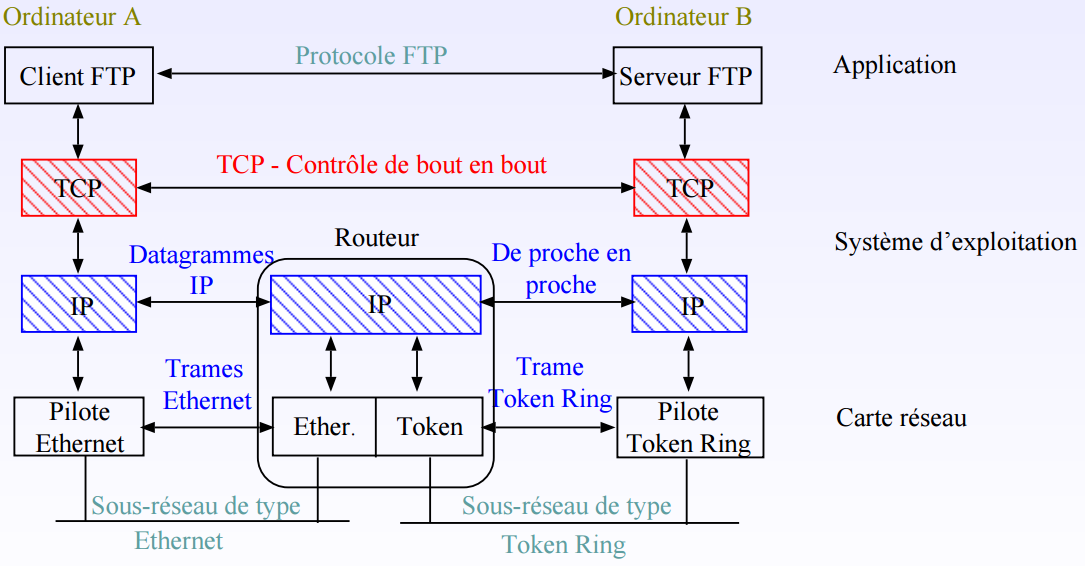
\includegraphics[width=\columnwidth]{hetero.png}
		\caption{Prise en compte de l'hétérogénéité}
		\label{fig:hetero}
		\end{center}
	\end{figure}
	
	\begin{figure}[!hbt]
		\begin{center}
		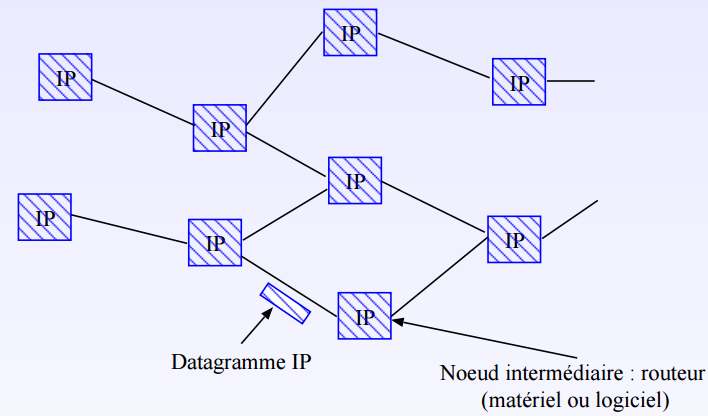
\includegraphics[width=\columnwidth]{comm.png}
		\caption{Couche réseau : communication entre machines}
		\label{fig:comm}
		\end{center}
	\end{figure}
	
	\subsection{Protocole IP}
	IP - Protocole d'interconnexion, best-effort
	\begin{itemize}
		\item acheminement de \textit{datagrammes} (mode \textit{non-connecté}
		\item peu de fonctionnalités
		\item pas de garanties, simple mais robuste (défaillance d’un noeud
intermédiaire)
	\end{itemize}
	
	\begin{figure}[!hbt]
		\begin{center}
		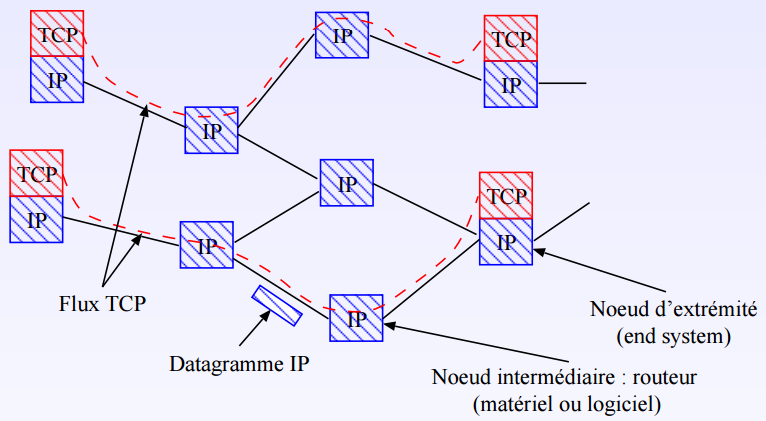
\includegraphics[width=\columnwidth]{comm2.png}
		\caption{Couche réseau : communication entre applications}
		\label{fig:comm2}
		\end{center}
	\end{figure}
	
	\subsection{Protocole TCP}
	TCP - Protocole de transport \textit{de bout en bout}
	\begin{itemize}
		\item uniquement présent aux \textit{extrémités}
		\item transport \textit{fiable} de \textit{segments} (mode \textit{connecté})
		\item protocole complexe (retransmission, gestion des erreurs, séquencement, ...)
	\end{itemize}
	
	\begin{figure}[!hbt]
		\begin{center}
		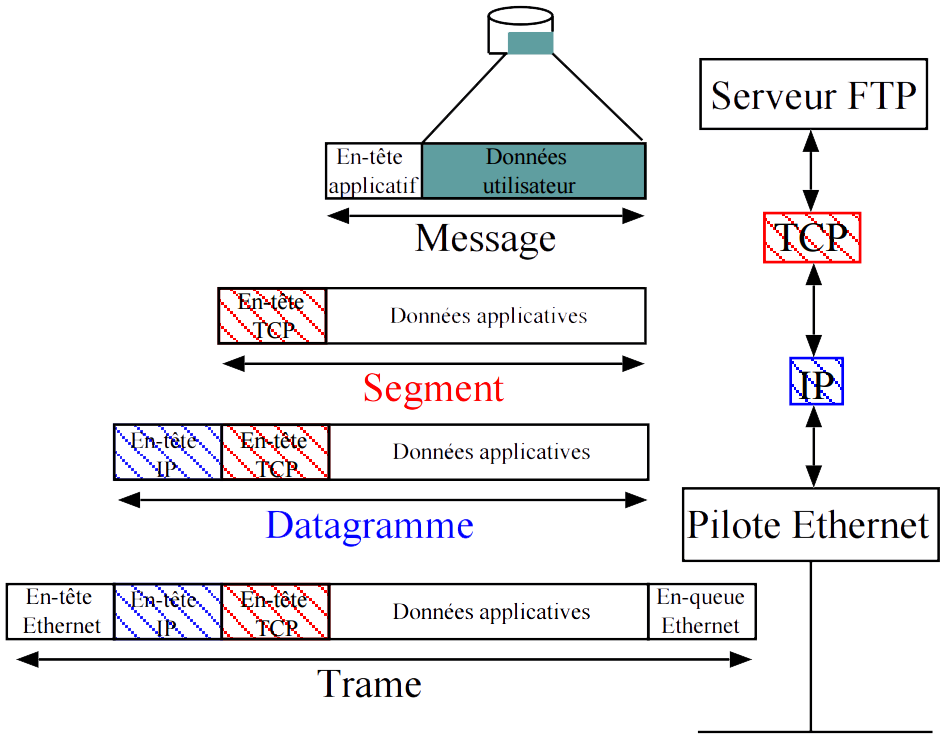
\includegraphics[width=\columnwidth]{archi_trame.png}
		\caption{Couche réseau : communication entre applications}
		\label{fig:archi_trame}
		\end{center}
	\end{figure}
	
	\begin{figure}[!hbt]
		\begin{center}
		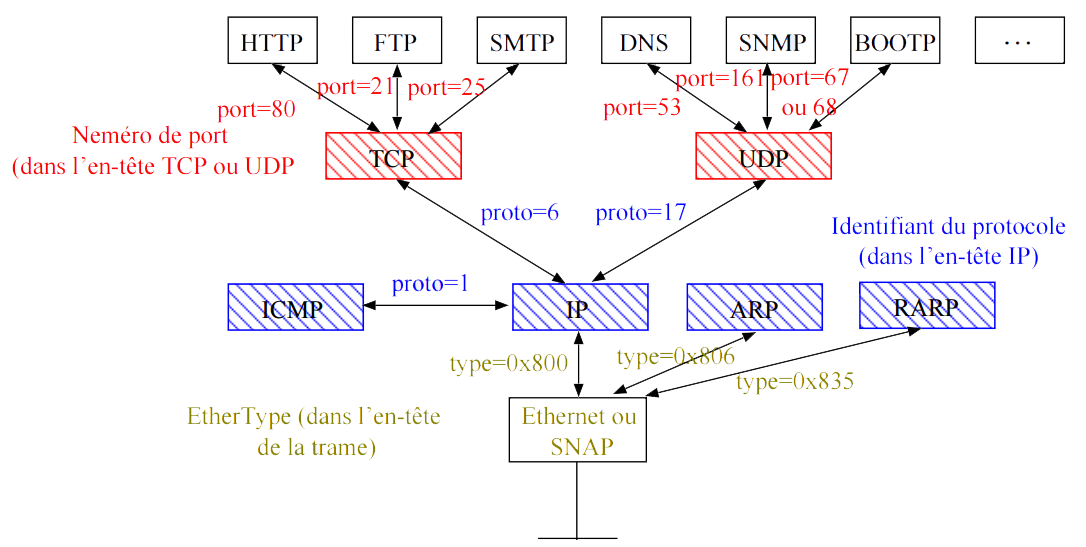
\includegraphics[width=\columnwidth]{id_proto.png}
		\caption{Identification des protocoles}
		\label{fig:id_proto}
		\end{center}
	\end{figure}
	
	\subsection{Identification des protocoles}
	\begin{itemize}
		\item Une adresse de transport = une adresse IP + un numéro de
port (16 bits) → adresse de socket
		\item Une connexion s’établit entre une socket source et une socket
destinataire → une connexion = un quintuplé (proto, src, port
src, dest, port dest)
		\item Deux connexions peuvent aboutir à la même socket
		\item Les ports permettent un multiplexage ou démultiplexage de
connexions au niveau transport
		\item Les ports inférieurs à 1024 sont appelés \textit{ports réservés}
	\end{itemize}
	
	\subsection{Protocole UDP}
	UDP (RFC 768) - User Datagram Protocol :
	
	\begin{itemize}
		\item protocole de transport le plus simple
		\item service de type best-effort (comme IP)
		\begin{itemize}
			\item les segments UDP peuvent être perdus
			\item les segments UDP peuvent arriver dans le désordre
		\end{itemize}
		\item  mode non connecté : chaque segment UDP est traité
indépendamment des autres
	\end{itemize}
	
	Pourquoi un service non fiable sans connexion ?
	
	\begin{itemize}
		\item simple donc rapide (pas de délai de connexion, pas d’état
entre émetteur/récepteur)
		\item petit en-tête donc économie de bande passante
		\item sans contrôle de congestion donc UDP peut émettre aussi
rapidement qu’il le souhaite
	\end{itemize}
	
	Les utilisations de l'UDP :
	
	\begin{itemize}
		\item Performance sans garantie de délivrance
		\item Souvent utilisé pour les applications multimédias
		\begin{itemize}
			\item tolérantes aux pertes
			\item sensibles au débit
		\end{itemize}
		\item Autres utilisations d’UDP
		\begin{itemize}
			\item applications qui envoient peu de données et qui ne nécessitent
pas un service fiable
			\item exemples : DNS, SNMP, BOOTP/DHCP
		\end{itemize}
		\item Transfert fiable sur UDP
		\begin{itemize}
			\item ajouter des mécanismes de compensation de pertes (reprise
sur erreur) au niveau applicatif
			\item mécanismes adaptés à l’application
		\end{itemize}
	\end{itemize}
	
	
	\subsection{Protocole TCP}
	Transport Control Protocol (RFC 793, 1122, 1323, 2018, 2581)
	Transport fiable en mode connecté :
	\begin{itemize}
		\item point à point, bidirectionnel : entre deux adresses de transport
(@IP src, port src) → (@IP dest, port dest)
		\item transporte un flot d’octets (ou flux)
		\begin{itemize}
			\item l’application lit/écrit des octets dans un tampon
		\end{itemize}
		\item assure la délivrance des données en séquence
		\item contrôle la validité des données reçues
		\item organise les reprises sur erreur ou sur temporisation
		\item réalise le contrôle de flux et le contrôle de congestion (à l’aide
d’une fenêtre d’émission)
	\end{itemize}
	
	\subsection{Exemples de protocole applicatif}
	\begin{itemize}
		\item HTTTP - HyperText Transport Protocol
		\begin{itemize}
			\item protocole du web
			\item échange de requête/réponse entre un client et u
serveur web
		\end{itemize}
		\item FTP - File Tranfer Protocol
		\begin{itemize}
			\item protocole de manipulation de fichiers distants
			\item tranfert, suppression, création, ...
		\end{itemize}
		\item TELNET - TELetypewriter Network Protocol
		\begin{itemize}
			\item système de terminal virtuel
			\item permet l'ouverture d'une session distante
		\end{itemize}
		\item DNS - Domain Name System
		\begin{itemize}
			\item assure la correspondance entre un nom
symbolique et une adresse Internet (adresse IP)
			\item bases de données réparties sur le globe
		\end{itemize}
	\end{itemize}
	
	\newpage

\section{Routage dans TCP/IP}

\subsection{Routage dans IP}

\subsubsection{Sous-réseaux}
~\\
Un sous-réseau est un sous-ensemble d'un réseau de classe.
Les intérêts d'un sous-réseau sont :
\begin{itemize}
	\item diviser un réseau de grande taille en plusieurs réseaux physiques connectés par des routeurs (locaux ou distants)
	\item possibilité de faire coexister des technologies de réseaux différents
	\item diminution de la congestion du réseau par redirection du traffic et réduction des diffusions
\end{itemize}
Pour créer ce sous-réseau, il faut un ID de sous-réseau en séparant les bits d'ID d'hôtes en plusieurs sections.
~\\
\subsubsection{Linux : Positionner/Modifier une adresse IP}
~\\
La manipulation des adresses IP se fait à l'aide de l'utilitaire \textit{ifconfig}.

Syntaxe :
\lstset{language=sh}
\begin{lstlisting}
ifconfig interface @IP netmask masque ...
\end{lstlisting}

Exemple (configuration de l'interface eth0) :
\begin{lstlisting}
ifconfig eth0 192.168.0.1 netmask 255.255.255.0
\end{lstlisting}
\subsubsection{Problématique du routage}
~\\
\textbf{Objectif} : Acheminer des datagrammes IP d’une machine source A vers une machine destination B.

\textbf{Problématique} : Commet atteindre la machine B en connaissant son adresse IP ?

\begin{figure}[!hbt]
	\begin{center}
	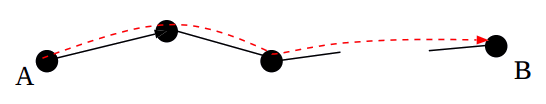
\includegraphics[width=\columnwidth]{routage.png}
	\label{fig:routage}
	\end{center}
\end{figure}

→ Nécessité d’identifier toutes les machines intermédiaires.
~\\
\subsubsection{Routage IP : principe de base}
~\\
Définition :
\begin{itemize}
	\item Processus de choix des chemins par lesquels les paquets sont transmis à la machine destinataire
	\item Processus basé sur une table de routage IP \textit{IP routing table} contenant les informations relatives aux différentes destinations possibles et à la façon de les atteindre
\end{itemize}

Principe de base :
\begin{itemize}
	\item L'émetteur ne connapit pas la route complète mais l'adresse du prochain site IP qui le rapprochera de la destination (prochain saut)
	\item Changements dynamiques possibles (en cas de panne)
	\item Extraire du datagramme l'adresse IP de destination (\textit{IPDest})
	\item Calculer l'adresse du réseau de destination (\textit{IPRes})
	\item Si \textit{IPRes} = \textit{IPLocal} alors
	\begin{itemize}
		\item \textit{IPDest} est directement accessible sur le réseau élémentaire commun
		\item La couche IP locale tente la translation d'adresse logique \textit{IPDest} en adresse physique à travers la table maintenue en cache
		\item Si le réseau est de type Ethernet, le protocole utilisé est ARP
		\item Sinon les adresses physiques destinataires X21 auront dû être configurées à la main au préalable
	\end{itemize}
	\item Sinon (ce n’est pas une adresse accessible, il faut alors consulter la table de routage IP locale) :
	\begin{itemize}
		\item Si \textit{IPRes} est dans la table alors :
		\begin{itemize}
			\item Router le datagramme selon les indications de la table (vers un autre nœud du réseau local, avec résolution adresse IP → adresse physique, ou vers un autre coupleur connecté à un réseau externe)
		\end{itemize}
		\item SInon \textit{IPRes} n'est pas dans la table alors :
		\begin{itemize}
			\item Prendre la route par défaut indiquée dans la table
			\item Router le datagramme selon les indications de l'entrée par défaut de la table (vers un autre nœud du réseau local, avec résolution d'adresse IP → adresse physique, ou vers un autre coupleur connecté à un réseau externe)
		\end{itemize}
	\end{itemize}
\end{itemize}
~\\
\subsubsection{Tables de routage IP dans Linux}
~\\
Afficher les routes :\\
\lstinline$~/# route$ ~\\
\lstinline$Destination     Gateway         Genmask     Iface$
\lstinline$default         10.3.255.254    0.0.0.0     wlan2$
\lstinline$10.3.0.0        *               255.255.0.0 wlan2$
~\\
~\\
Ajouter une route par défaut :\\
\lstinline$~/# route add defaut gw @passerelle$ 
~\\
~\\
Ajouter une route utilisatn l'interface réseau \textit{iface} vers un hôte particulier) :\\
\lstinline$~/# route add -host @host gw @passerelle dev iface$
~\\
~\\
Ajouter une route utilisant l'interface \textit{iface} vers un réseau particulier :\\
\lstinline$~/# route add -net @reseau netmask mask dev iface gw @gw$
~\\
~\\
Pour les suppression de route, il suffit de remplacer \lstinline$add$ par \lstinline$del$.

\subsubsection{Mise en place d'un réseau}
~\\
\textbf{Concentrateur (hub)} : partage de bande passante entre les hôtes raccordés.
\textbf{Commutateur (switch)} : pas d'interférences entre les connexions simultanées.
\textbf{Routeur} : Pas d'interférences entre des connexions simultanées, possibilité de communication entre 2 réseaux logiques différents.

\newpage
\section{Réseaux privés}

\subsection{Introduction}

Les adresse privées ont été crées pour :
\begin{itemize}
	\item gérer la pénurie d'adresses au sein d'un réseau
	\item masquer l'intérieur d'un réseau par rapport à l'extérieur
	\item améliorer la sécurité pour le réseau interne
\end{itemize}

Il existe 2 mécanismes de translation d'adresses (NAT - Network Address Translation) :
\begin{itemize}
	\item \textbf{statique} : association entre \textit{n} adresses publiques et \textit{n} adresses privées
	\item \textbf{dynamique} : association entre \textit{1} adresse publique et \textit{n} adresses privées
\end{itemize}

\subsection{NAT statique}

Intérêt :
\begin{itemize}
	\item Uniformité de l'adressage dans la partie privée du réseau (modif. de la correspondance @pu/@pri facile)
	\item Sécurité accrue (tout passe par la passerelle NAT)
\end{itemize}

L'inconvénient majeur est que la pénurie d'@pu n'est pas résolue.
	
\begin{figure}[!hbt]
	\begin{center}
	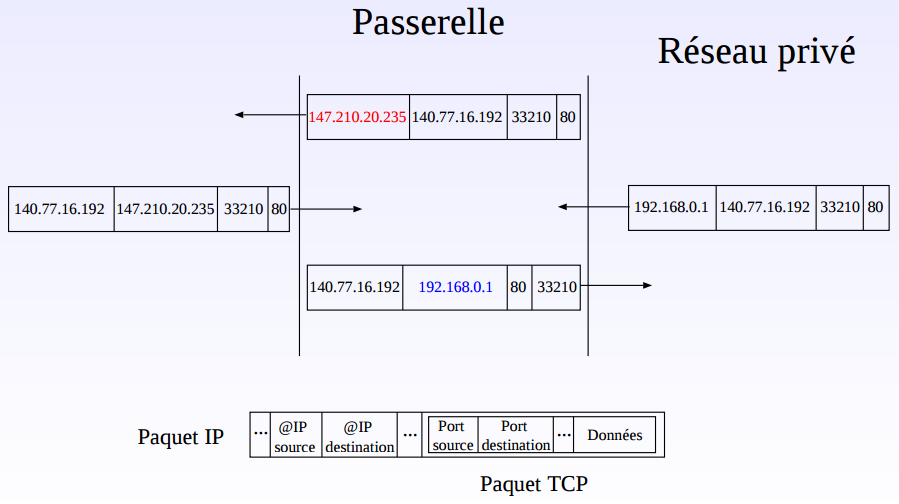
\includegraphics[width=\columnwidth]{nat_stat.png}
	\caption{NAT statique : principe de fonctionnement}
	\label{fig:nat_stat}
	\end{center}
\end{figure}

\subsection{NAT dynamique : Masquerading}

Intérêt :
\begin{itemize}
	\item Plusieurs machines utilisent la même @pu pour sortir du réseau privé
	\item Sécurité accrue (tout passe par la passerelle NAT)
\end{itemize}

L'inconvénient majeur est que les machines du réseau interne ne sont pas accessibles de l'extérieur (impossible d'initier une connexion de l'extérieur).
\newpage

\subsubsection{Fonctionnement}
~\\
Comment le routeur fait-il la diférence entre les paquets qui lui sont destinés et les paquet à relayer :

\begin{lstlisting}
A chaque nouvelle connexion :
  Modif. @src et port source:
  (@src_pri,port_src)->(@pu,port_src)
  Sauvegarder l'asso ds table NAT
Pour chaque paquet entrant :
  Chrcher une asso. (@dest., port_dest)
  Si exist une asso. ds table NAT Alors :
    Modif. (@dest., port_dest)
    Relayer le paquet
  Sinon
    /*Erreur de routage*/
  FinSi
\end{lstlisting}

Le routeur gère toutes les associations, il y a donc unicité de l'association (donc du port source après translation).
~\\
\subsubsection{Problèmes liés à NAT dynamique}
~\\
\begin{itemize}
	\item Nécessité d'implémenter une méthode spécifique aux protocoles n'utilisant pas de port
	\item Protocoles utilisant @IP, nécessité de mettre en place un "\textit{proxy}" (\textsc{FTP} en mode actif par exemple)
	\item Nécessité de faire de la redirection de port (port mapping/forwarding)
\end{itemize}

~\\
\subsubsection{Proxy}
~\\
Un proxy est un intermédiaire dans une connexion entre le client et le serveur.\\
Le client s'adresse toujours au proxy.\\
Le proxy est spécifique à une application donnée (\textsc{HTTP}, \textsc{FTP}, ...).
	
\begin{figure}[!hbt]
	\begin{center}
	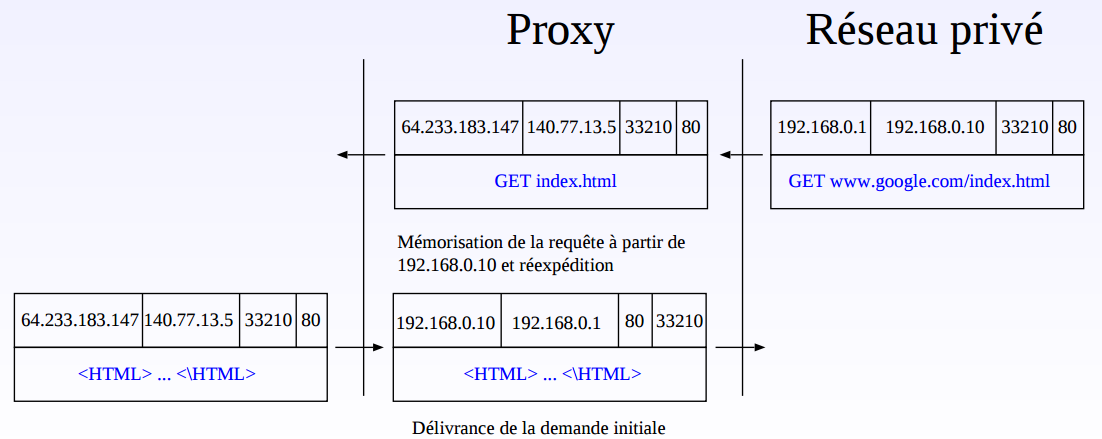
\includegraphics[width=\columnwidth]{proxy.png}
	\caption{NAT statique : principe de fonctionnement}
	\label{fig:proxy}
	\end{center}
\end{figure}

\newpage
\section{Iptables et NAT}

La fonctionnalité de \textit{firewall} est implémentée dans le noyau de Linux. Il y a 3 type de firewall filtrant :
\begin{itemize}
	\item \textit{ipfwadm} : jusqu’à la version 2.1.102 du noyau linux
	\item \textit{ipchains} : entre les versions 2.2.0 et 2.4 du noyau linux
	\item \textit{iptables} : à  partir des noyaux 2.4
\end{itemize}

Nous nous intéresserons seulement à \textit{iptables} dans ces notes de cours, car c'est la version que nous avons utilisé en TP. Se référer au cours complet pour avoir des informations sur les autres firewalls.

3 types de règles :
\begin{itemize}
	\item \textbf{INPUT} : sont appliquées lors de l’arrivée d’un paquet
	\item \textbf{FORWARD} : sont appliquées lorsque la destination du paquet n'est pas le routeur
	\item \textbf{OUTPUT} : sont appliquées dès qu'un paquet doit sortir du routeur
\end{itemize}

\begin{figure}[!hbt]
	\begin{center}
	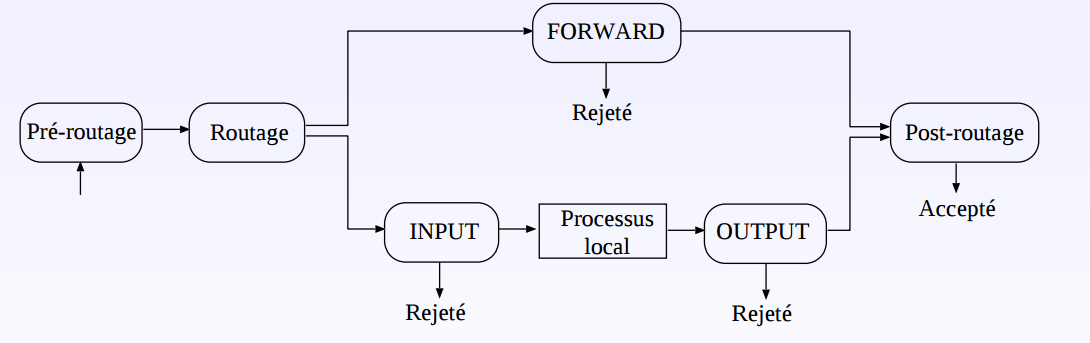
\includegraphics[width=\columnwidth]{iptables_fonct.png}
	\caption{\textit{iptables} : principe de fonctionnement}
	\label{fig:iptables_fonct}
	\end{center}
\end{figure}

A chaque table une fonctionnalité :
\begin{itemize}
	\item \textit{filter} : filtrage des paquets
	\item \textit{nat} : NAT
	\item \textit{mangle} : marquage des paquets
\end{itemize}
~\\
\begin{tabular}{|p{1.7cm}|p{1.9cm}|p{2.5cm}|p{1.9cm}|}
  \hline
  \multicolumn{2}{|c|}{\textsc{FILTER}} & \multicolumn{2}{c|}{\textsc{NAT}} \\
  \hline
  \textsc{INPUT} & paquet entrant sur le routeur & \textsc{PREROUTING} & NAT de destination \\
  \hline
  \textsc{OUTPUT} & paquet émis par le routeur & \textsc{POSTROUTING} & NAT de source \\
  \hline
  \textsc{FORWARD} & paquet traversant le routeur & \textsc{OUTPUT} & NAT sur les paquets émis localement \\
  \hline
\end{tabular}
\newpage
\subsection{Fonctionnalités NAT}

\begin{figure}[!hbt]
	\begin{center}
	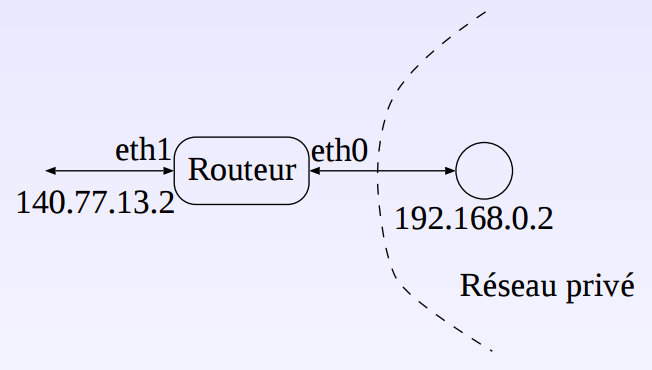
\includegraphics[width=\columnwidth]{iptables_nat.png}
	\caption{\textit{iptables} : NAT statique}
	\label{fig:iptables_nat}
	\end{center}
\end{figure}

Arrivée d'un paquet de l'extérieur :\\
\textit{iptables -t nat -A PREROUTING -d 140.77.13.2 -i eth1 -j DNAT −−to-destination 192.168.0.2}\\
~\\
Paquet émis depuis le réseau privé :\\
\textit{iptables -t nat -A POSTROUTING -s 192.168.0.2 -o eth1 -j SNAT −−to-source 140.77.13.2}\\
~\\
2change de paquet entre le routeur et la machine du réseau privé :\\
\textit{iptables -t nat -A OUTPUT -d 140.77.13.2 -j DNAT −−to-destination 192.168.0.2}

\begin{figure}[!hbt]
	\begin{center}
	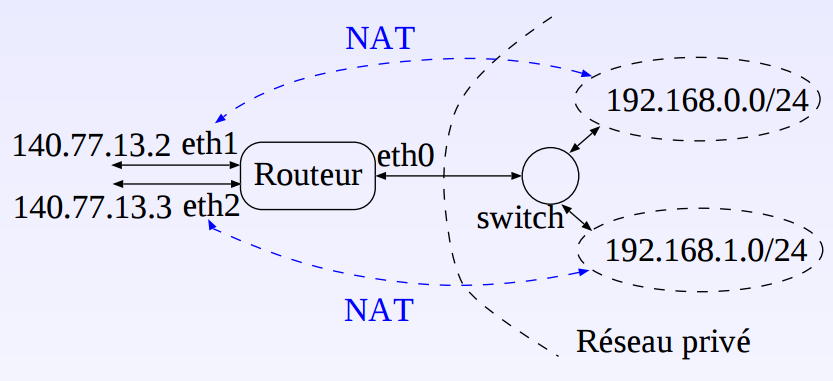
\includegraphics[width=\columnwidth]{iptables_nat_dy.png}
	\caption{\textit{iptables} : NAT dynamique}
	\label{fig:iptables_nat_dy}
	\end{center}
\end{figure}

Association entre toutes les adresses privées du sous-réseau 192.168.0.0/24 avec l’interface eth1 :\\
\textit{iptables -t nat -A POSTROUTING -o eth1 -s 192.168.0.0/24 -j MASQUERADE}\\
~\\
Association entre toutes les adresses privées du sous-réseau 192.168.1.0/24 avec l’interface eth2 :\\
\textit{iptables -t nat -A POSTROUTING -o eth2 -s 192.168.1.0/24 -j MASQUERADE}\\
~\\
Transférer les connexions sur le port 80 de l’adresse 140.77.13.2 sur la machine ayant l’adresse privée 192.168.0.200 sur le port 8080 :\\
\textit{iptables -t nat -A PREROUTING -p tcp -d 140.77.13.2 −−dport 80 −−sport 1024:65535 -j DNAT −−to 192.168.0.200:8080}


\newpage
\section{Firewall}

Pourquoi un firewall ?
\begin{itemize}
	\item Contrôle (des connexions sortantes)
	\item Sécurité (contre les intrusions externes)
	\item Vigilance (surveiller/tracer le trafic entre le réseau local et internet)
\end{itemize}

Il y a plusieurs type de firewall :
\begin{itemize}
	\item Niveau réseau (iptables, paquet filter, ...)
	\item Niveau applicatif (inetd, xinetd, ...)
	\item Niveau des applications (/etc/ftpaccess pour ftp, ...)
\end{itemize}

\subsection{DMZ}

Une zone démilitarisée (DMZ) est un sous-réseau se trouvant entre le réseau local et le réseau extérieur.

Propriétés :
\begin{itemize}
	\item Les connexions à la DMZ sont autorisées de n’importe où
	\item Les connexions à partir de la DMZ ne sont autorisées que vers l’extérieur
\end{itemize}

Intérêt :
\begin{itemize}
	\item Rendre des machines accessible à partir de l’extérieur (possibilité de mettre en place des serveurs (DNS, SMTP, ...)
\end{itemize}

\subsection{iptables et filtrage}

Les règles sont traitées de manière séquentielle : le paquet sort dès qu'il rencontre une règle qui peut lui être appliquée.

~\\
\subsubsection{Exemples d'utilisation}
~\\
Accepter tous les paquets en provenance de n’importe où et destinés à l’adresse du routeur 192.168.1.1 :\\
\textit{iptables -A INPUT -s 0/0 -i eth0 -d 192.168.1.1 -p TCP -j ACCEPT}\\
~\\
Accepter de router les paquets entrant sur eth0 tels que (@src : 0/0, @dest : 192.168.1.58, P-source : 1024-65535, P-dest : 80) :\\
\textit{iptables -A FORWARD -s 0/0 -i eth0 -d 192.168.1.58 -o eth1 -p TCP −−sport 1024:65535 −−dport 80 -j ACCEPT}\\
~\\
Accepter un paquet ICMP “echo-request” (ping) par seconde :\\
\textit{iptables -A INPUT -p icmp −−icmp-type echo-request -m limit −−limit 1/s -i eth0 -j ACCEPT}

\subsection{iptables et suivi des connexions}

Il y a 4 états possibles  pour une connexion :
\begin{itemize}
	\item \textbf{NEW} : nouvelle connexion établie
	\item \textbf{ESTABLISHED} : la connexion analysée est déjà établie
	\item \textbf{RELATED} : la connexion est en relation avec une connexion  déjà établie (ftp-data par exemple)
	\item \textbf{INVALID} : le paquet reçu n'appartient à aucune des trois catégories précédentes
\end{itemize}

~\\
\subsubsection{Exemples d'utilisation}
~\\
Autoriser tous les paquets émis par le routeur concernant des connexions déjà établies :\\
\textit{iptables -A OUTPUT -o eth0 -m state −−state ESTABLISHED,RELATED -j ACCEPT}\\
~\\
Autoriser le routeur à relayer tous les paquets reçus concernant de nouvelles connexions sur le port 22 :\\
\textit{iptables -A FORWARD -p tcp -i eth0 −−dport 22 −−sport 1024:65535 -m state −−state NEW -j ACCEPT}\\

\newpage
\section{Révision annales}
~\\
\textbf{Rôle du daemon portmap} :\\
Conversion des numéros de programme RPC (Remote Procedure Call) en numéro de port.
~\\
~\\
\textbf{Quelle est la différence entre une résolution itérative et une résolution récursive en DNS ?}\\
\begin{itemize}
	\item \textit{Itérative} : la machine qui demande la résolution de nom contacte un serveur DNS et attend que ce dernier lui retourne la réponse désirée.
	\item \textit{Récursive} : le serveur de noms contacté fournit en réponse le nom d’un autre serveur DNS à contacter pour avancer dans la résolution.
\end{itemize}
~\\
\textbf{A quoi sert le champ MX dans les zones DNS, donnez un exemple d'utilisation de ce dernier}\\
Les enregistrements Mail Exchange (MX) dirigent les e-mails d'un domaine vers les serveurs hébergeant les comptes utilisateur du domaine. Plusieurs enregistrements MX peuvent être définis pour un même domaine, chacun avec une priorité différente. Si un e-mail ne peut être distribué à l'aide de l'enregistrement associé à la priorité la plus élevée, l'enregistrement de priorité 2 est utilisé, etc.
~\\
~\\
Exemple : \textit{dig labri.fr. MX}
~\\
~\\
\textbf{Expliquez le fonctionnement du protocole DHCP, pourquoi ce mécanisme est-il basé sur un mécanisme de \textit{broadcast} ?}\\
\begin{figure}[!hbt]
	\begin{center}
	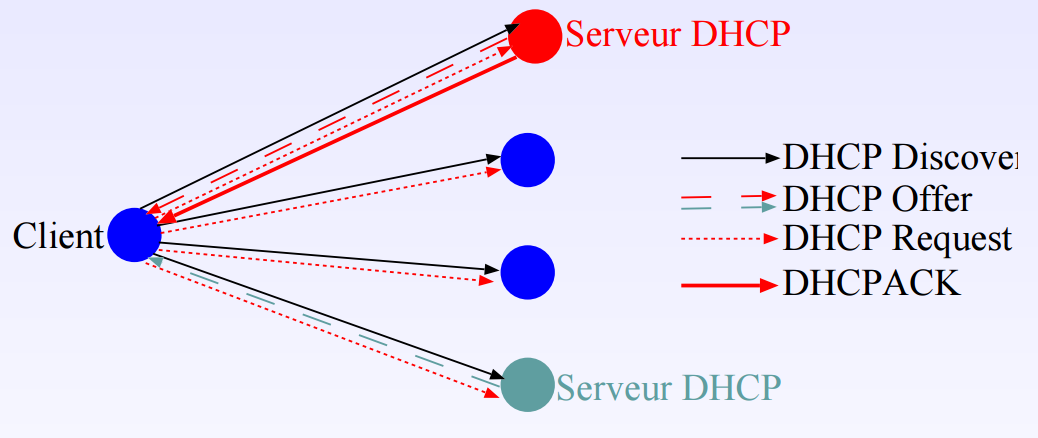
\includegraphics[width=\columnwidth]{dhcp.png}
	\label{fig:dhcp}
	\end{center}
\end{figure}
\begin{itemize}
	\item Discover : le client diffuse un broadcast avec son @MAC, à la recherche du serveur, sur les ports 68/UDP (client) et 67/UDP (serveur)
	\item Offer : le serveur choisit une configuration pour le client (pouvant se baser sur l'@MAC du client
	\item Request : le client choisi une config et la précise dans son message
	\item Acknowledge : Confirmation du serveur + éventuellement bail
\end{itemize}
\newpage
\textbf{Différence LDAP et NIS ?}\\
~\\
\begin{tabular}{|p{2cm}|p{2cm}|p{2cm}|}
\hline
~ 				& \textbf{LDAP} 				& \textbf{NIS}\\
\hline
\hline
Mot de passe	& Crypté 						& Non-crypté\\
\hline
Redondance		& Uniquement dans le serveur	& Distribué à chaque client/serveur esclave\\
\hline
Fonction		& Beaucoup d'infos (UID, adresse, ...) & Seulement l'identifiant et le mot de passe\\
\hline
\end{tabular}
~\\
~\\
\textbf{Dans LDAP, donner deux points illustrant l'intérêt d'utiliser le mécanisme de réplication}\\
~\\
\begin{itemize}
	\item Tolérance aux pannes (en cas de crash d'un serveur)
	\item En cas de saturation d'un serveur
\end{itemize}
~\\
~\\
\textbf{Quelles sont les propriétés d'une DMZ ?}\\
Une zone démilitarisée (DMZ) est un sous-réseau se trouvant entre le réseau local et le réseau extérieur.
~\\
\textit{Propriétés :}
\begin{itemize}
	\item Les connexions à la DMZ sont autorisées de n’importe où
	\item Les connexions à partir de la DMZ ne sont autorisées que vers l’extérieur
\end{itemize}
~\\
\textit{Intérêt :}
\begin{itemize}
	\item Rendre des machines accessible à partir de l’extérieur (possibilité de mettre en place des serveurs (DNS, SMTP, ...)
\end{itemize}
~\\
~\\
\textbf{Expliquer le principe de la résolution DNS. Il est demandé de considérer les deux cas suivants : le serveur de nom local connaît la réponse, le serveur de nom local ne connaît pas la réponse.}\\
\begin{itemize}
	\item \textit{Le serveur local connaît la réponse :} il retourne la réponse au client.
	\item \textit{Le serveur local ne connaît pas la réponse :} selon la configuration :
	\begin{itemize}
		\item Récursif : le serveur va demander à un autre serveur la réponse
		\item Itératif : le serveur renvoie au client l'adresse d'un autre serveur à qui demander
	\end{itemize}
\end{itemize}
~\\
~\\
\textbf{Quel est le point commun entre NIS et NFS ? Qu'implique l'utilisation de ce mécanisme ?}\\
Le point commun est qu'ils utilisent tous les deux portmap, et l'utilisation de ce mécanisme entraîne donc l'utilisation de la correspondance numéro de programme RPC / numéro de port.
~\\
~\\
\textbf{Expliquer rapidement le fonctionnement du protocole ARP.}\\
\begin{figure}[!hbt]
	\begin{center}
	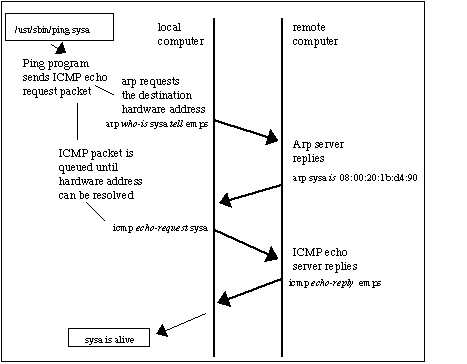
\includegraphics[width=10cm]{arp.png}
	\label{fig:arp}
	\end{center}
\end{figure}
~\\
~\\
\textbf{Qu'apporte l'utilisation de caches dans les protocoles tels qu'ARP ou DNS ? Quels sont les problèmes posés par l'utilisation de tels caches ?}\\
Elle permet d'éviter une con-gestion (c'est su verlant) du serveur en ayant les réponses dans ce cache et en plus ça permet de gagner du temps à éviter de lancer des requêtes sur des autres serveurs.\\
Le problème est que ce cache peut-être modifié et donc le serveur fournira des fausses informations.
~\\
~\\
\textbf{Expliquer le fonctionnement de la translation d'adresses dynamique.}\\
Le routeur modifie l'adresse source d'un paquet sortant et l'adresse de destination d'un paquet entrant. Il n'y a qu'une adresse publique pour \textit{n} clients. Le routeur retrouve la machine du réseau selon le port source donné pour le flux sortant.
% Your document ends here!
\end{document}